\section{Fission}
\label{sec:fission}


\begin{figure*}[t!]
\centering
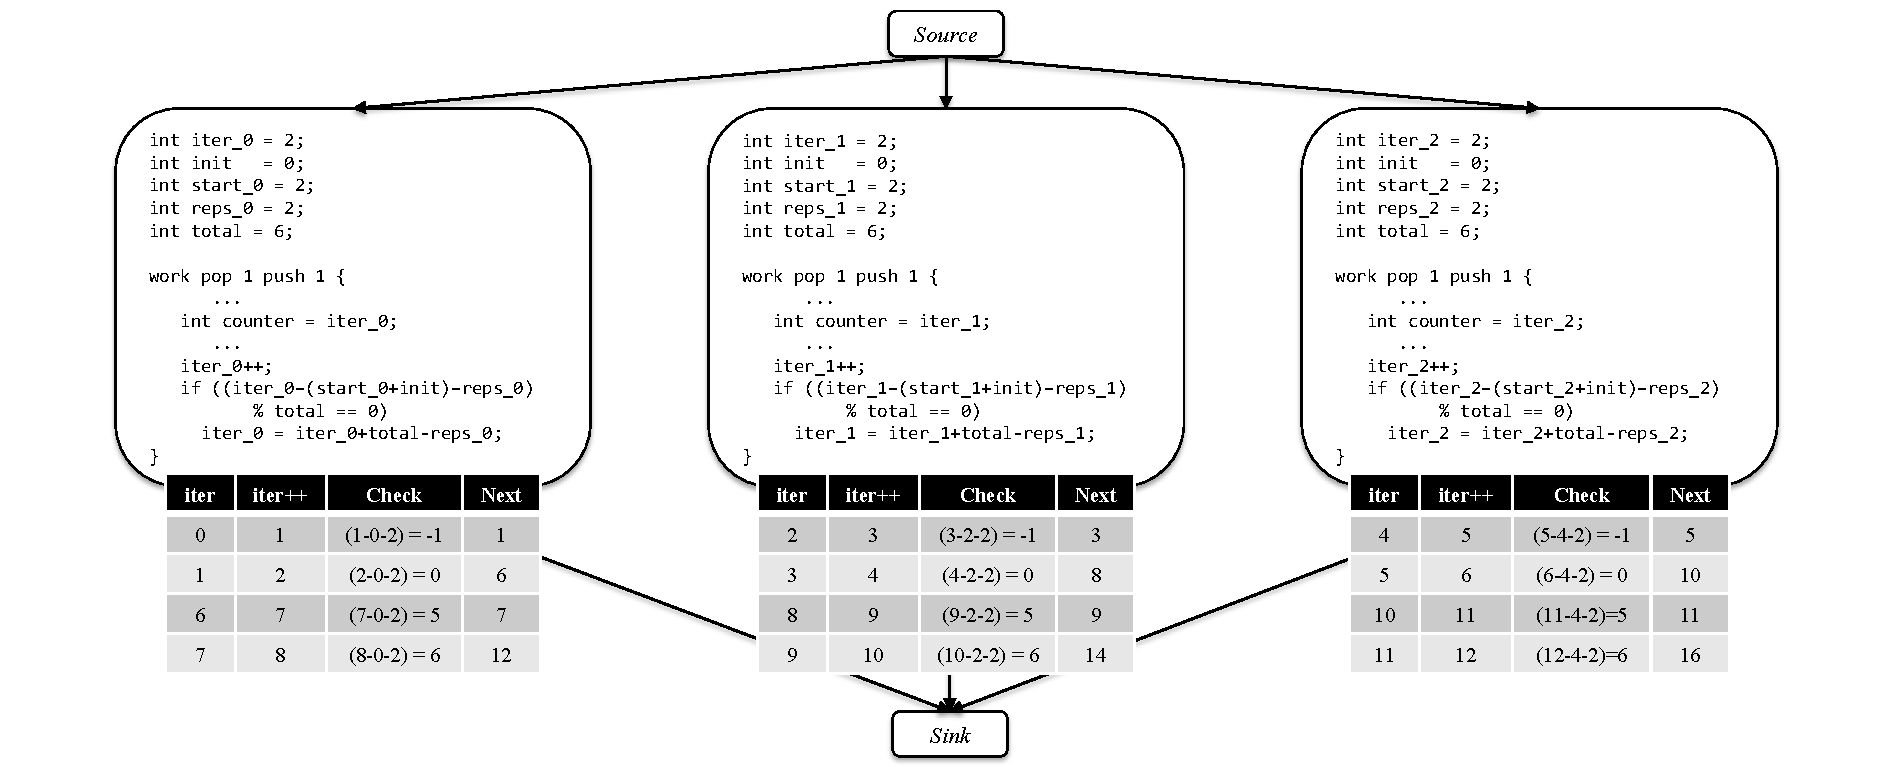
\includegraphics[width=6.5in]{figures/fission-example.pdf}
\caption{.\protect\label{fig:fission-example}}
\end{figure*}


The compiler introduces data parallelism to the streaming program through a process known as fission.  Fission is the process of duplicating the stateless filter and wrapping these duplicated in a round-robin splitter and joiner.  The process ensures that input data is distributed correctly and output data is collected in correct order.  The duplicated filters, known as products, can be assigned to individual cores, thus introducing data parallelism.  

Fission is applicable only to stateless filters, as the duplication process does not guarantee consistent behavior if filters contain state that changes between iterations.  Because the desugared iteration filters actually use mutable state to keep track of iteration values, the fission process must be modified to handle iteration values.  

\begin{figure}[t]
{\eightpoint
\begin{verbatim}
  int->int filter IterationFilter() {

      int iter = 0;
      int start = 0;
      int reps = 1;
      int total = 10;

      work push 1 pop 1{

          ...

          iter++;

          if (iter - start - reps % total == 0) {
              iter = iter + total - reps;
          }

      }

  }
\end{verbatim}
\caption{Example of a duplicated iteration filter under modified fission.\protect\label{fig:modified-fission-filter-example}}}
\end{figure}


The fission process now modifies the fission products by adding the
following values as fields of the products:
\begin{itemize}
    \item \texttt{start}: the value of the induction variable each product starts with.
    \item \texttt{reps}: how often the \texttt{work} function of the product is
      called between rounds.
    \item \texttt{total}: the sum of all reps of all fission products. This value is
      the same amongst all fissed products.
\end{itemize}
Accordingly, each fission product should start each round with induction values
of
\begin{center}
\texttt{total}*\texttt{n} + \texttt{start}
\end{center}
and range up to the value
\begin{center}
\texttt{total}*\texttt{n} + \texttt{start} + \texttt{reps} - 1
\end{center}
where \texttt{n} is a nonnegative integer indicating how many rounds have
been run in the span of the program.  We have to account for the off-by-one
error as the first iteration is run.

The \texttt{start} value of every fissed product must also take the initialization schedule into account.  Initialization execution of the original filter is transferred entirely to the first fission product.  Accordingly, \texttt{start} for the first fission product indicates the multiplicity of the initialization schedule.  All subsequent fission products have \texttt{start} as the sum of all multiplicities of prior fission products and the multiplicity of the initialization schedule.

At the end of each fission product \texttt{work}, after incrementing the
induction value, a check must be made to see if it is necessary to increment
the induction variable to the next round of  values.  This will prevent certain
fissed products from making calls with duplicate induction values.
\begin{center}
\texttt{iter} - \texttt{start} - \texttt{reps} \% \texttt{total} == 0
\end{center}
The fissed products must check that the current induction value less the
\texttt{start} and \texttt{reps} of that fissed product is divisible by the
\texttt{total}.  This is consistent with the maximum value per round as
indicated above.  Once the fissed product's induction value has reached
this value, it must be set to:
\begin{eqnarray*}
\texttt{iter}_{n+1} &=& \texttt{iter}_{n} + (\texttt{total} - \texttt{reps}) \\
&=& (\texttt{total}*\texttt{n} + \texttt{start} + \texttt{reps}) \\
&&  \ \ +\ (\texttt{total} - \texttt{reps}) \\
&=& (\texttt{total}*(\texttt{n+1}) + \texttt{start})
\end{eqnarray*}
which is the starting iteration value of the next round, as defined.

Future passes may modify the schedule, increasing the multiplicity of the fission products.  All of the fission products will have this multiplicity applied. It is necessary to multiply the iteration constants by the provided multiplier.

Given a multiplier $m$, we expect the filter to start each round with iteration values of 
\begin{center}
(\texttt{total}*\texttt{n} + \texttt{start}) * $m$
\end{center}
The filter should perform \texttt{reps}*$m$ iterations, thus should range up to value
\begin{center}
(\texttt{total}*\texttt{n} + \texttt{start}) * $m$ + \texttt{reps}*$m$ - 1
\end{center}

Between rounds, iteration values must be incremented by the actual total number of repetitions that occur.  All fission products perform a total of $\sum(\texttt{reps}_{i}*m)$ repetitions which is simply \texttt{total}*$m$.  Thus, the updating step will still hold:
\begin{eqnarray*}
\texttt{iter}_{n+1} &=& \texttt{iter}_{n} + (\texttt{total}*m - \texttt{reps}*m) \\
&=& (\texttt{total}*\texttt{n}*m + \texttt{start}*m + \texttt{reps}*m) \\
&&  \ \ +\ (\texttt{total}*m - \texttt{reps}*m) \\
&=& (\texttt{total}*(\texttt{n+1})*m + \texttt{start}*m)
\end{eqnarray*}

